\documentclass[a4paper,11pt]{article}
\usepackage{xcolor}
\usepackage{tikz}
\usepackage{tkz-euclide}
\usetikzlibrary{intersections,shapes.arrows,arrows.meta}
\begin{document}
\def\radius{6mm}
\begin{figure}[H]
	\begin{center}
		\scalebox{0.4}{
			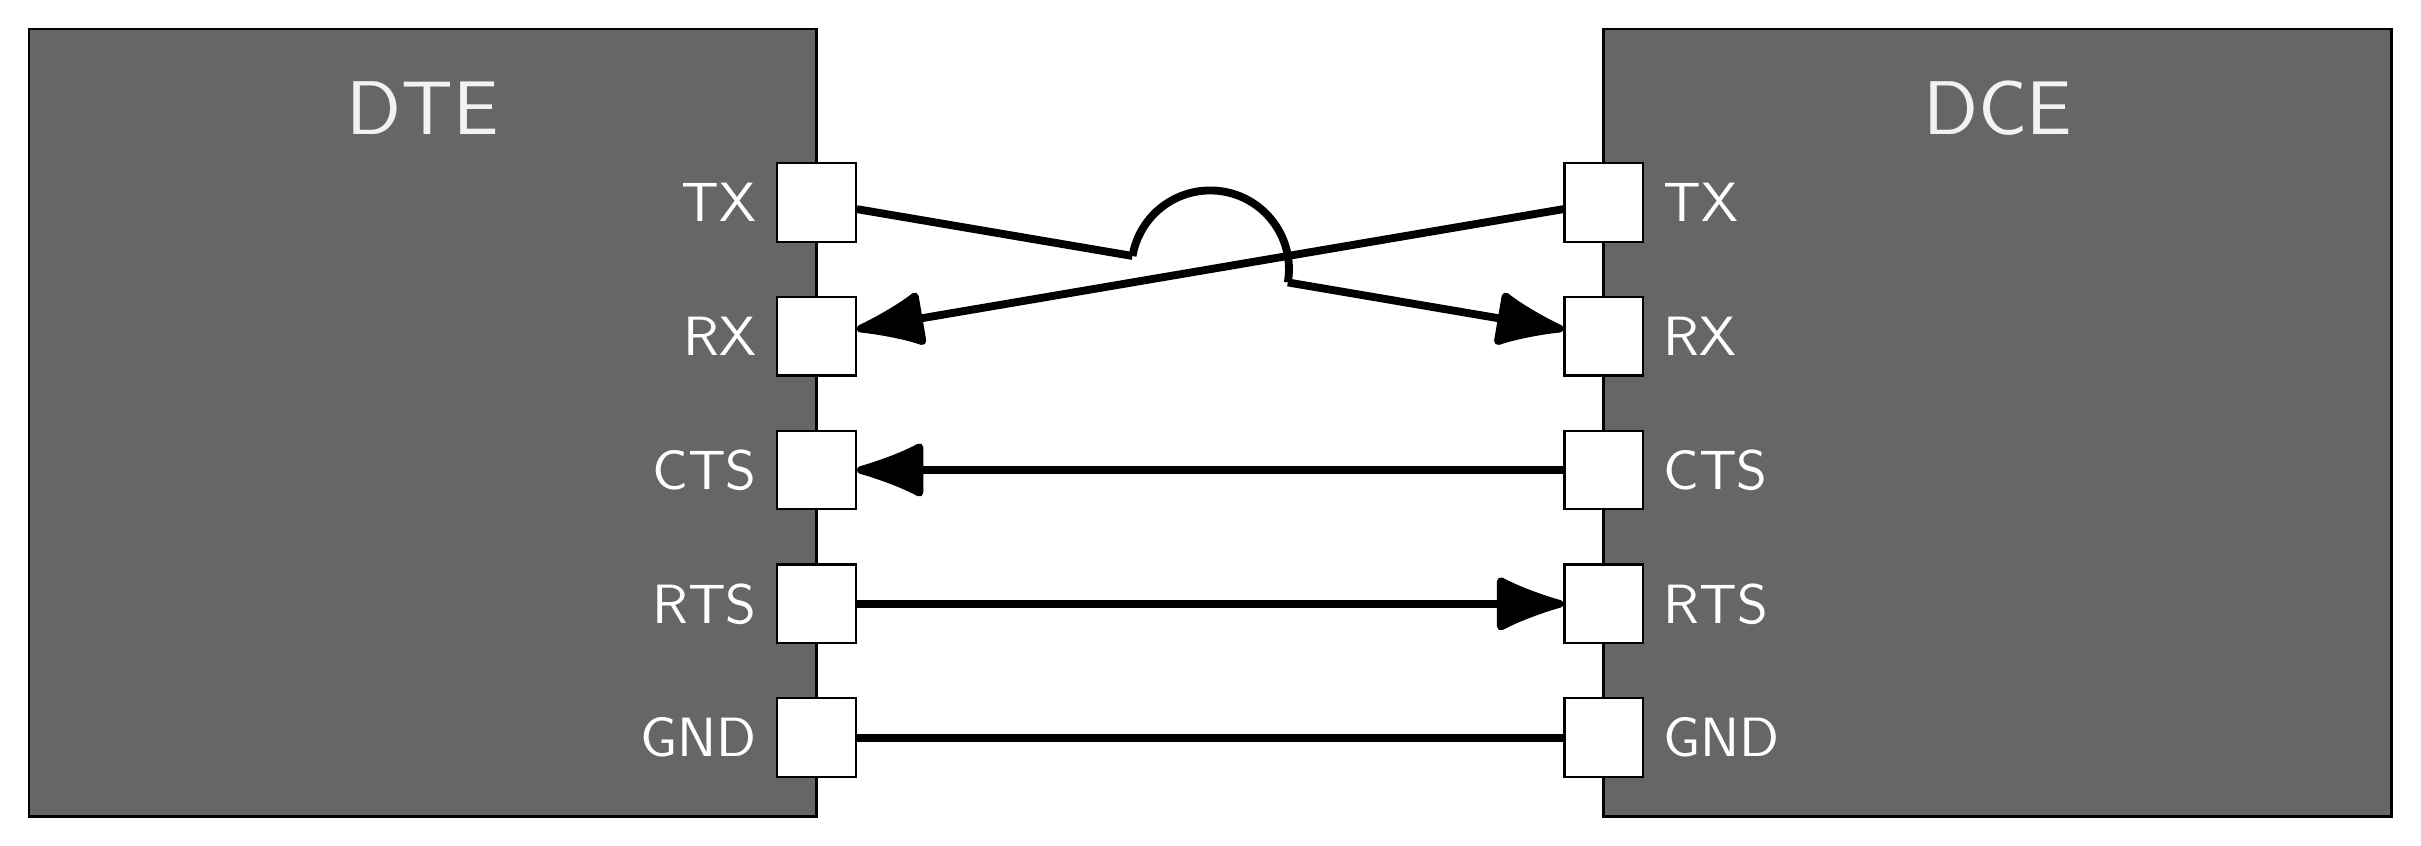
\begin{tikzpicture}[font=\sffamily]
				\draw[line width=1, fill=black!60] (0,0) rectangle ++(10,10);
				\draw[line width=1, fill=black!60] (20,0) rectangle ++(10,10);
				\draw (5,9) node[scale=2.75,black!5]{DTE};
				\draw (25,9) node[scale=2.75,black!5]{DCE};

				\foreach \p [count=\q from 0] in {{GND},{RTS},{CTS},{RX},{TX}}{
					\node (rect) at (10, 1+\q*1.7) [draw,thick,minimum width=1cm,minimum height=1cm,fill=white,label={[white,scale=2] left:\p}] (l-\p){};
					\node (rect) at (20, 1+\q*1.7) [draw,thick,minimum width=1cm,minimum height=1cm,fill=white,label={[white,scale=2] right:\p}] (r-\p){};
				}

	\draw [-{Latex[length=1cm, round]},line width=1mm,name path=line 1] (r-TX) -- (l-RX);
\path[name path=line 2] (l-TX) -- (r-RX);
\path [name intersections={of = line 1 and line 2, name=i}];
\coordinate (S) at (i-1);
\path[name path=c1] (S) circle(\radius);
\path [name intersections={of = c1 and line 2, name=i}];
\coordinate (I1)  at (i-2);
\coordinate (I2)  at (i-1);
\draw[line width=1mm] (l-TX) -- (I2);
\draw[-{Latex[length=1cm, round]},line width=1mm] (I1) -- (r-RX);
			\tkzDrawArc[line width=1mm](S,I1)(I2);

				\draw [line width=1mm,{Latex[length=1cm, round]}-] (l-CTS) -- (r-CTS);
				\draw [line width=1mm,-{Latex[length=1cm, round]}] (l-RTS) -- (r-RTS);
				\draw [line width=1mm] (l-GND) -- (r-GND);

			\end{tikzpicture}
		}
		\caption{Legacy hardware flow control.}
		\label{fig:legacyctl}
	\end{center}
\end{figure}
\end{document}



